\clearpage
\section{Literature Review}
\label{sec:LitReview}

\subsection{Clustering Time Series Gene Expression Values}

Clustering techniques are essential in the data mining process, as they reveal natural structures and identify interesting patterns in the underlying data.

For gene expression data observed at different time-points, clustering can help identify biologically relevant groups of genes and samples.

Through the principle of guilt-by-association \cite{quackenbush2003microarrays}, if we find a significant cluster with some uncharacteristic genes, we can hypothesize that these genes are also significant.

As mentioned in \cite{d2005does}, there is no one-size-fits-all solution to clustering, or even a consensus of what an ideal clustering should be like. Clusters may have arbitrary shapes and sizes, and each clustering criterion imposes a certain structure on the data. If the data happen to conform to the requirements of a particular criterion, the true clusters are recovered, however, very rarely is this the case. Each algorithm imposes its own set of biases on the clusters it determines. Most (reasonable) clustering algorithms would yield similar results on synthetically constructed datasets; however, in practice, they can give widely differing results on real-world,noisy, gene expression data.

For temporal gene expression data, the most commonly used clustering algorithms are \cite{friedman2000using,jiang2004cluster,schliep2003using} are
\begin{enumerate}
    \item Model Based Clustering
    \begin{itemize} 
        \item K-Means 
        \item Gaussian Mixture Models
        \item Hidden Markov Models
        \item Bayesian Networks
    \end{itemize}
    \item Hierarchical Clustering
    \item Self Organizing Maps
\end{enumerate}

For all our model based clustering techniques, we determine partitions by using the expectation-maximization (EM) algorithm (described in \ref{EM}) for maximum likelihood estimates of model parameters .

In this report, we will use hierarchical clustering for exploratory analysis, and apply all the model based clustering techniques to the different datasets we are provided with.


\subsection{Algorithms and Models}

\subsubsection{Expectation Maximization (EM) Algorithm}
\label{EM}

The expectation maximization (EM) algorithm is a general technique for finding maximum likelihood solutions for probabilistic models having latent variables \cite{bishop2006pattern}. EM is used for all the model based techniques covered in this report. 
\simpleparagraph{Procedure}

Consider a probabilistic model in which we collectively denote all the observed variables by $\mathbf{X}$ and the hidden variables by $\mathbf{Z}$. The join distribution is governed by a set of parameters, denoted $\theta$. We try to maximize the likelihood function, that is given by 
\begin{equation}
    p(\mathbf{X}|\theta) = \sum_{\mathbf{Z}} p(\mathbf{X},\mathbf{Z} | \theta)
\end{equation}
If $\mathbf{Z}$ is continuous, we replace the summation with integration as appropriate.
The maximum likelihood estimator is 
\begin{equation*}
    \theta = \argmin_{\theta} f(\theta)
\end{equation*}
Direct optimization of $p(\mathbf{X}|\theta)$ is difficult due to the presence of latent variables, so we attempt to optimize the expected value of the log-likelihood of the data given our model. We are now ready to define the general EM algorithm.
\begin{algorithm}[h]
\caption{Expectation Maximization}
\small
        \item \textbf{Initialization:} For $l=0$, make an initial estimate of the parameters $\theta$.
        \item \textbf{E Step ($l^{th}$ iteration):} Evaluate  p(\mathbf{Z}|\mathbf{X},$\theta$), i.e find the conditional probability distribution of the latent variables given our current model $\theta^{(l)}$ and the data \mathbf{X}.
        \item \textbf{M Step ($l^{th}$ iteration):} Update $\theta$ as
        \begin{equation}
            \theta^{(l+1)} = \argmin_{\theta} u(\theta, \theta^{(l)}
        \end{equation}
        where 
        \begin{equation}
            u(\theta, \theta^{(l)}) = 
            - \sum_{\mathbf{Z}} p(\mathbf{Z}| \mathbf{X},\theta^{(l)}) \log p(\mathbf{X},\mathbf{Z}|\theta) 
            + \sum_{\mathbf{Z}} p(\mathbf{Z}| \mathbf{X},\theta^{(l)}) \log p(\mathbf{Z}|\mathbf{X},\theta^{(l)})
        \end{equation}
        \item \textbf{End:} Terminate when one of the following criteria is met
        \begin{enumerate}
            \item Iterate till $l$ reaches the maximum number of iterations specified
            \item Till the parameter estimates stop changing
            \item Till the likelihood function stop changing
        \end{enumerate}
\end{algorithm}

\paragraph{Limitations}

The EM Algorithm typically converges to the local optima. Thus, it needs to be run multiple times in order to find the best fitting model and its parameters.

\subsubsection{K-Means}

K-Means is an algorithm to identify groups, or clusters, of data points in a multidimensional space \cite{bishop2006pattern}. 

We group data points based on their feature similarities according to a given distance metric (Euclidean Distance in our case), by minimizing a given cost function. 

Given a set of data points $D = \{x_t\}^n_{t=1}$ and fixed number of clusters $K \leq n$, the algorithm works as follows \cite{TanVYF}:-

\begin{algorithm}[h]
\caption{K-Means Clustering}

        \item \textbf{Step 0, Initialization:} For $j=1,..,K$, initialize centers ${\mu_j}^{(1)}$ randomly.
        \item \textbf{Step $l \in \mathbb{N}$, Assignment (E) Step:} Assign each point $x_t$ to its closest mean
        \begin{equation*}
            {j_t}^{(l)} = \argmin_j {||x_t-\mu_j||}^2
        \end{equation*}
        \item \textbf{Step $l \in \mathbb{N}$, Update (M) Step:} Recompute $\mu_j$'s as means of the assigned points:
        \begin{equation*}
            \mu_j^{(l+1)} = \frac{1} { | \{ t : j_t^{(l)} =j\}|} \sum_{t : j_t^{(l)}=j} {x_t}
        \end{equation*}
        \item \textbf{End:} Terminate when cluster assignments $j_t$ don't change.
    
\end{algorithm}

For a given partition $D = \cup_{j=1}^{K} D_j$,
where 
\begin{equation*}
    D_j:= \{ x \in D : j = \argmin_{j} ||x-\mu_j'||^2 \}
\end{equation*}
this algorithm minimizes the overall squared error:
    \begin{equation}
        J(D_1,\dots,D_n,\mu_1,\dots,\mu_n)
        = \sum_{j=1}^K \sum_{x \in D_j}{{||x - \mu_j||}^2}
    \end{equation} \label{eq:k_means_cost}
where $D_1,D_2,\dots,D_n$ are the clusters and $\mu_1,\mu_2,\dots,\mu_n$ are cluster means. The two steps of updating the clusterings and re-estimating the centers correspond to the E step and M step of the EM Algorithm respectively.

Equation \eqref{eq:k_means_cost} is also known as the cost function.

The main problem of k-means is its dependency on the initially chosen centers. If the centers are chosen arbitrarily, then the algorithm converges very slowly or results in poor clustering. However, this can be solved by using the \textbf{K-Means++} \cite{arthur2007k} algorithm, which selects centers that are far apart from each other in a probabilistic manner. 

Through K-Means++, we choose the initial $K$ centers as follows \cite{TanVYF}:-

\begin{enumerate}
    \item Take a random data point $\mu_1$ chosen uniformly from dataset $D$.
    \item Calculate new center $\mu_i$, by choosing $x \in D$ with probability $\frac{D(x)^2}{\sum_{x' \in D} D(x')^2}$, (where $D(x)$ denotes the shortest distance from the data point $x$ to its closest, already chosen center)
    \item Repeat the previous step till we have $K$ centers.
\end{enumerate}

\paragraph{Limitations}
Due to its ease of implementation and termination in a finite number of steps, K-Means is one of the most popular (and usually one of the first) algorithms applied for unsupervised learning problems. 

However, due to the nature of the distance function chosen (Euclidean), K-means doesn't capture temporal dependencies in the data. Thus, it is not entirely suitable for our time series dataset. Moreover, k-means does hard clustering, i.e. a point can belong to only one cluster, while in real life data, a point can belong to more than one cluster.

\subsubsection{Gaussian Mixture Models}

Gaussian mixture models (GMMs) are mixtures, or linear combinations, of models with Gaussian distributions. They are widely used in data mining, statistical analysis and pattern recognition problems \cite{bishop2006pattern}. 

\begin{figure}[h]
    \centering
    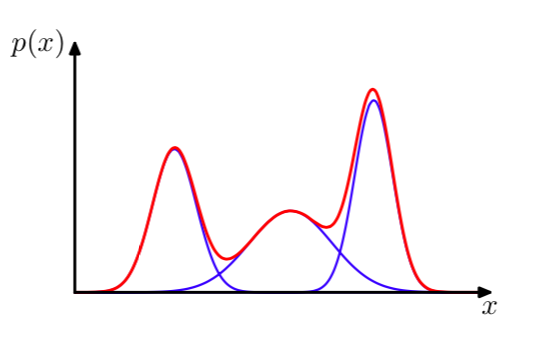
\includegraphics[width=0.5\textwidth]{Figures/GMM.png}
    \caption{Mixture of 3 Gaussians in one dimension}
    \label{fig:GMM}
\end{figure}

A Gaussian mixture model is represented by 
\begin{equation} \label{eq: GMM}
    p(\mathbf{x)} = \sum_{k=1}^{K} \pi_k \mathcal{N} ( \mathbf{x} | \mu_k, \Sigma_k)
\end{equation}

where the equation above represents a mixture of $K$ Gaussians, $\mathcal{N} ( \mathbf{x} | \mu_k, \Sigma_k)$ is a \textit{component} of the mixture model (each having its own mean $\mu_k$ and covariance $\Sigma_k$, and $\pi_k$ are the component weights, such that $\sum_k \pi_k = 1$.

To use GMMs for clustering, we assume that our data are generated i.i.d from a mixture of $K$ Gaussians, and we apply EM to estimate the $K$ means, covariances, and weights, and thus determine the clusterings. We achieve this by introducing a latent variable $z$ in \eqref{eq: GMM}. This latent variable has a 1-of-K representation - thus $z_k \in \{0,1\}$ and $\sum_k z_k=1$, and find $p(\mathbf{z})$ and $p(\mathbf{x|z})$, to get
\begin{equation} \label{eq: GMM_latent}
    p(\mathbf{x)} = \sum_z p(\mathbf{z})p(\mathbf{x|z})= \sum_{k=1}^{K} \pi_k \mathcal{N} ( \mathbf{x} | \mu_k, \Sigma_k)
\end{equation}
where $p(\mathbf{z}) = \displaystyle \prod_{k=1}^{K} \pi_k^{z_k}$ and $p(\mathbf{x|z}) = \displaystyle \prod_{k=1}^{K} \pi_k^{z_k} \mathcal{N} ( \mathbf{x} | \mu_k, \Sigma_k)^{z_k} $. 

Another quantity that is important is the conditional probability of $\mathbf{z}$ given $\mathbf{x}$, also known as the \textit{responsibility} that component $k$ takes for producing the observation $\mathbf{x}$, denoted by 

\begin{equation} \label{eq:respons}
    \gamma(z_k) = p(z_k = 1|x) = \frac{\pi_k \mathcal{N}(x|\mu_k,\Sigma_k)}{\sum_{j=1}^{K} \pi_j \mathcal{N} (x|\mu_j, \Sigma_j)}
\end{equation}

These formulas containing latent variable $z$ help us formulate EM for GMM, given in \ref{alg:EMGMM}.

\begin{algorithm} [h]
\caption{EM for Gaussian Mixture Models}
\label{alg:EMGMM}
        \item \textbf{Init}: Initialize the means and covariances $\mu_k$ and $\Sigma_k$ and mixing co-efficients $\pi_k$, and evaluate the initial value of the log-likelihood.
        \item \textbf{Step l, E step}: Evaluate the responsibilities from \eqref{eq:respons} using the current parameter values.
        \item \textbf{Step l, M Step}: Re-estimate the parameters using the current responsibilities.
        \begin{equation*}
             \mu_k^{(l+1)} = \frac{1}{N_k} \sum_{n=1}^{N} \gamma(z_{n,k}) \mathbf{x}_n 
             \end{equation*}
             \begin{equation*}
                             \Sigma_k^{(l+1)} = \frac{1}{N_k} \sum_{n=1}^{N} \gamma(z_{n,k}) (\mathbf{x}_n - \mu_k^{(l+1)})(\mathbf{x}_n - \mu_k^{(l+1)})^T
        \end{equation*}
        \begin{equation*}
            \pi_k^{(l+1)} = \frac{N_k}{N}
        \end{equation*}
        where $N_k = \sum_{n=1}^N \gamma(z_{nk})$
        \item Evaluate the log-likelihood
        \begin{equation*}
            \log p(X|\mu,\Sigma, \pi) = \sum_{n=1}^N \log \{ \sum_{k=1}^K \pi_k \mathcal{N} (x_n|\mu_k,\Sigma_k) \}
        \end{equation*}
        and \textbf{terminate} if one of the following criteria are met- 
        \begin{enumerate}
            \item Paramater estimates have converged (stopped changing).
            \item Log likelihood has converged.
            \item Maximum umber of iterations $l$ have been reached.
        \end{enumerate}
        otherwise return to Step 2.
\end{algorithm}

The clusterings are indicated by the latent variable $\mathbf{z}$.

\newpage
\paragraph{Covariance Matrix}
Having different settings of the covariance matrix for each component help in restricting the number of parameters that need to be estimated (thus optimizing the runtime of the algorithm). However, some of the settings (diagonal, tied and spherical) restrict the contour of the clusters obtained, as seen in figure \ref{fig:Covariance}. In the diagonal setting, the elliptical clusters obtained are aligned with the co-ordinate axes, while the spherical clusters are circular, while all clusters have the same shape in the tied setting. Assuming we have $k$ components, here are 4 different covariance settings, summarized in the table \ref{tab:GMM_Cov}. 
\begin{table}[h]
    \centering
    \begin{tabular}{|c|c|c|}
        \hline
         \textbf{Covariance} & \textbf{Description} & \textbf{Parameters} \\    \hline

         Full & \pbox{20cm}{\hspace{0.1cm}\\Each component has its own \\ general covariance matrix\\} & \small $\frac{KD(D+1)}{2}$ \\     \hline

         Diagonal& \pbox{20cm}{\hspace{0.1cm}\\Each component has a\\ diagonal covariance matrix\\} & $KD$\\    \hline

         Spherical & \pbox{20cm}{\hspace{0.1cm}\\Each component \\ has a single variance\\} & $K$\\    \hline

         Tied & \pbox{20cm}{\hspace{0.1cm}\\All components share the\\ same general covariance matrix\\} &  $\frac{D(D+1)}{2}$\\   \hline

    \end{tabular}
    \caption{Covariance Settings for GMM}
    \label{tab:GMM_Cov}
\end{table}

\begin{figure}[h]
    \centering
    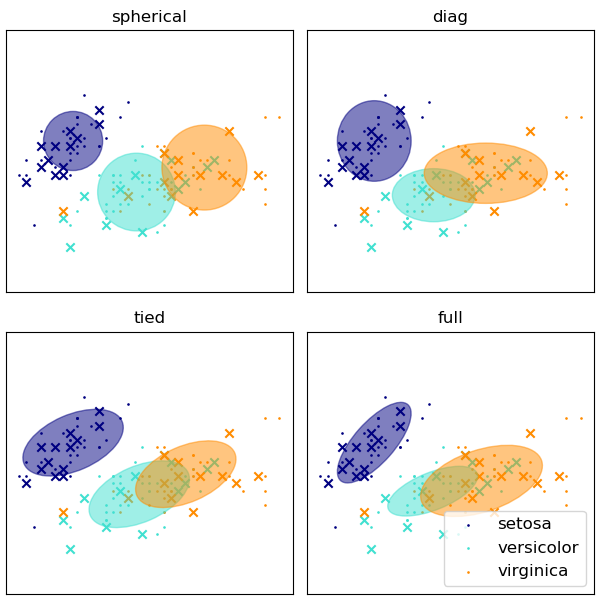
\includegraphics[width = 0.45\textwidth]{Figures/Covar.png}
    \caption{Different covariance settings for the 2D Iris dataset}
    \label{fig:Covariance}
\end{figure}
\paragraph{Limitations}
As discussed for previous models, GMM converges to a local optima, so we need to run the model multiple times to determine the best fit. Moreover, GMM takes a long time to run - however, we can indicate different parameter settings for the covariance matrix, based on what we know (or assume) about the data. This helps keeps the number of parameters that we are estimating under control and reduces the computation time.

\subsubsection{Hidden Markov Models}

\subsubsection{Bayesian Networks}

In \cite{TanVYF}, we studied the Chow-Liu algorithm to learn  tree-structured graphical models. In \cite{pham2009unsupervised}, the authors combined Chow-Liu Trees and Expectation Maximization to derive a model-based clustering method, called the CL Multinet Classifier.

If there are $K$ classes, then $K$ CL trees are learned. Each tree distribution $Pr_k$ approximates the joint probability distribution of the attributes, given a specific class. The root attribute has no parents, while the other attributes can have at most ONE parent, i.e. if the attributes are expressed as r.vs $\{X_1, X_2,...,X_n\}$, then $\Pi_{X_i} = \{X_{j \neq i}\}$ has only one attribute, and $\Pi_{X_{root}} = \{\emptyset\}$. 
 
Using Bayes Theorem, the posterior probability of a Chow Liu Tree can be expressed as
 \begin{equation}
         Pr(C=k|X_1,X_2,...,X_n) =\frac{ Pr(C=k)Pr(X_1,X_2,...,X_n|C=k)}{\sum_{k'}Pr(C=k')Pr(X_1,X_2,...,X_n | C = k')}
 \end{equation}
We observe that the denominator is constant with respect to the class, so we express it as $\frac{1}{\beta}$. 
 
Then, the previous formula can be re-written as
 
\begin{equation}
    Pr(C=k|X_1,X_2,...,X_n) = \beta*Pr(C=k)\prod_{i=1}^{n} Pr_k(X_i | \Pi_{X_i})
\end{equation}
 
The edge weights of a Chow Liu tree are encoded by the \textit{mutual information}, which is derived from the empirical probability distributions observed from the data.
 
 \begin{equation}
     I(X,Y) = \sum_{x \in X} \sum_{y \in Y} Pr(x,y) \log \frac{Pr(x,y)}{Pr(X)Pr(y)}
 \end{equation}
 
 A maximum weighted spanning tree (either Prim's/Kruskal's) algorithm is then used to find the Chow-Liu tree for each $k^{th}$ class.
 
 Unsupervised training of the CL Trees (henceforth referred to as CL Multinets) is carried out assuming that the data have been generated from a mixture of $K$ Bayesian networks. This mixture can be described as 
 \begin{equation}
     Pr(X) = \sum_{k=1}^{K} \alpha_k f_k(X)
 \end{equation}
where 
\begin{equation}
    \sum_{k=1}^{K} \alpha_k = 1, \hspace{0.5cm}\alpha_k \geq 0
\end{equation}

The $\alpha_k$ are the mixing coefficients and the $f_k$ are the joint probability distributions of the CL Multinets.
 \simpleparagraph{EM Procedure}
 Given $N$ observations, $K$ clusters (CL Multinets), and initial partitions P$^0$=\{P$_0^0$,P$_1^0$,...,P$_K^0$\}, the EM procedure for the $m^{th}$ iteration is as follows:
 \begin{itemize}
     \item E-Step: For $r=1,2,...,N$ and $k=1,2,...,K$ compute the posterior probabilities for $x^r$ belonging to P$_k$.
     \begin{equation}
         t_k^m(x') = \frac{\alpha_k^m \prod_{i=1}^{n} Pr_k^m(x_i^r|\Pi_{x_i^r})}{\sum_{k'=1}^{K}\alpha_{k'}^m \prod_{i=1}^{n} Pr_{k'}^m(x_i^r | \Pi_{x_i^r})}
     \end{equation}
     \item C-Step: Update the partition $P^m$=\{P$_0^m$,P$_1^m$,...,P$_K^m$\} by assigning each $x^r$ to the cluster that provides the max posterior probability.
     \item M-Step: For $k=1,...,K$, maximize the Classification Maximum Likelihood (CML) criteria and re-estimate the parameters $\theta^m$ using the new partitions $P_k^m$.
     \begin{equation} \label{eq:CML}
         CML = \sum_{k=1}^{K}\sum_{x^r \in P_k} \log \prod_{i=1}^{n} Pr_k(x_k^r | \Pi_{x_i^r}) + \sum_{k=1}^{K} n_k \log \alpha_k
     \end{equation}
      where $n_k$ are the number of samples belonging to the $k^{th}$ cluster, and $\alpha_k$ are the cluster weights.
      
      The parameters for the second term are re-estimated (maximized) using the following formula:
      \begin{equation}
          \alpha_k^{m+1} = \frac{n_k}{N}, \hspace{0.5cm} k=1,...,K
      \end{equation}
      
      The first term (after some manipulation) contains the mutual information computed by the observed data (empirical distributions). Using the maximum weighted spanning tree algorithm, we maximize \eqref{eq:CML}, resulting in a new tree distribution.
\end{itemize}

\paragraph{Limitations}
Although Bayesian Networks are directed acyclic graphs and thus use fewer parameters than HMMs, unlike HMMs, we need to discretize the data in order to use the empirical frequencies to estimate joint probability distributions. Discretization also results in loss of information, as the resultant dataset is dependent upon the number of bins chosen. Moreover, just like HMM-based clustering, there exist only general information theoretic criteria to determine the number of clusters $K$, which is not always be applicable \cite{pham2009unsupervised}.

\subsubsection{Hierarchical Clustering}

All the previous models that we covered can be classified under \textit{partitional clustering}. The other category, hierarchical clustering, seeks to build a hierarchy of clusters using a given distance metric for datum and a similarity criteria for the clusters obtained. However, unlike partitional clustering, there exist no definitive statistical techniques determine the optimal number of clusters - instead, we need to examine the resulting hierarchical structure (dendogram) and visually determine the optimal number of clusters \cite{maimon2005data}.
 
 There are two approaches to hierarchical clustering - 
 \begin{itemize}
     \item Agglomerative: Each datum initially represents a cluster of its own. Clusters are then successively merged until the desired cluster structure is obtained.
     \item Divisive: All objects initially belong to one cluster. This main cluster is then divided into sub-clusters, which are successively sub-divided into their own sub-clusters, and this process continues until the desired cluster structure is obtained.
 \end{itemize}
 
For this report, we use agglomerative hierarchical clustering \textit{not} in model building, but in our initial exploratory analysis, so as to obtain a rough estimate of the number clusters we may expect from the data.

We set the distance metric (for within cluster distances) as Euclidean. 
The linkage criterion in hierarchical clustering specifies the difference between any two sets obtained. It determines which clusters to merge by calculating the differences between two clusters as a function of the pairwise distances between observations. The different types of linkages are-
\begin{itemize}
    \item Single: the distance between two clusters is equal to the shortest distance from any member of one cluster to any member of the other cluster. 
    \item Average: the distance between two clusters is equal to the average distance from any member of one cluster to any member of the other cluster.
    \item Complete: the distance between two clusters is equal to the longest distance from any member of one cluster to any member of the other cluster.
    \item Ward: the distance is defined as the error function of the unified cluster minus the error functions of the individual clusters, where the error function is the average distance of each data point in a cluster to the cluster centroid.
\end{itemize}

\begin{figure}
    \centering
    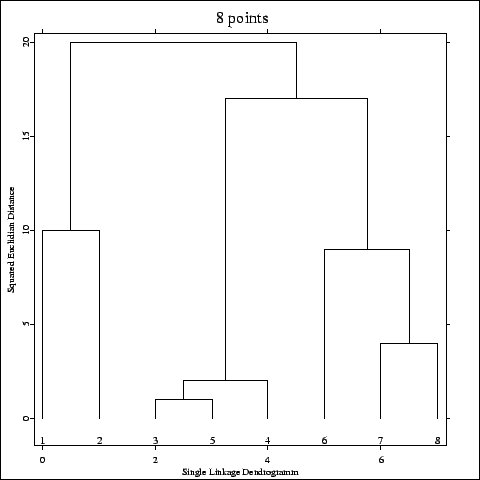
\includegraphics[width=0.6\textwidth]{Figures/hier.png}
    \caption{Hierarchical Clustering Dendogram for Single-Linkage}
    \label{fig:HC}
\end{figure}
\subsection{Evaluation Metrics for Model Selection}

Given data, model selection is the task of selecting the best statistical model from a set of candidate models. 

In our clustering analysis, the main conundrum is determining the number of clusters.

The estimation of the true number of classes has been recognized as “one of the most difficult problems in cluster analysis" \cite{bock1996probabilistic}. The correct choice of $K$ is often ambiguous - sometimes, choosing the best fitting model is not the wisest choice. Consider increasing $K$ without any penalty - this will keep reducing the error but the model is less than ideal (e.g. In K-Means, if we have $n$ clusters for $n$ points, each point is its own center, reducing the cost function to 0). 

Moreover, given multiple candidate models having similar accuracy, the simplest model is most likely to be the best choice (Occam's razor).

Thus, the optimal choice of $K$ balances accuracy and number of parameters required for the model. This is tackled in \ref{conundrum1} and \ref{con1}.

A secondary conundrum is comparing two different clustering models, given that we obtain "ground truth" values for some of the clusters. This is handled in \ref{condundrum2}. 
\subsubsection{Information Theoretical Methods} \label{conundrum1}

When a statistical model is used to represent the process that generated the data, the representation will almost never be exact. Some information is thus lost by the model. Bayesian Information Criteria (BIC) and Akaike Information Criteria (AIC) \cite{burnham2004multimodel} deal with estimating this lost information, and calculate the trade-off between the \textit{goodness of fit} of the model and the \textit{complexity} of the model.

\paragraph{BIC and AIC}

BIC and AIC penalize the total number of parameters. Both are functions of the maximized log-likelihood of the model and the estimated number of parameters - however, BIC penalizes model complexity more heavily. We define the AIC and BIC as follows:-

\begin{equation*}
    AIC =  \log L(\theta) - P \\
\end{equation*}

\begin{equation*}
        BIC =  \log L(\theta) - \frac{P}{2}\log(N) 
\end{equation*}

where $L(\theta)$ is the maximized log-likelihood of the model $\theta$, $P$ is the number of free parameters and $N$ is the number of data points. For a range of $K$ values, we calculate AIC/BIC, and choose the $K$ for which this criterion is \textit{maximum}. Thus, higher AIC or BIC values indicate better fitting models. 



\subsubsection{Elbow Method}\label{con1}
The elbow method \cite{kodinariya2013review} is a popular method to determine the true number of clusters by plotting the cost function for a given clustering algorithm against different $K$, and observing the point where the graph makes a sharp \textit{elbow} shape, as seen in Figure \ref{fig:elbow}. More formally, this method looks at the percentage of variance explained as a function of the number of clusters. In essence, the elbow method observes the point of sharpest decrease in the cost function, i.e. the most improvement to the cost function, and estimates that to be the ideal number of clusters.
\begin{figure}[h]
    \centering
    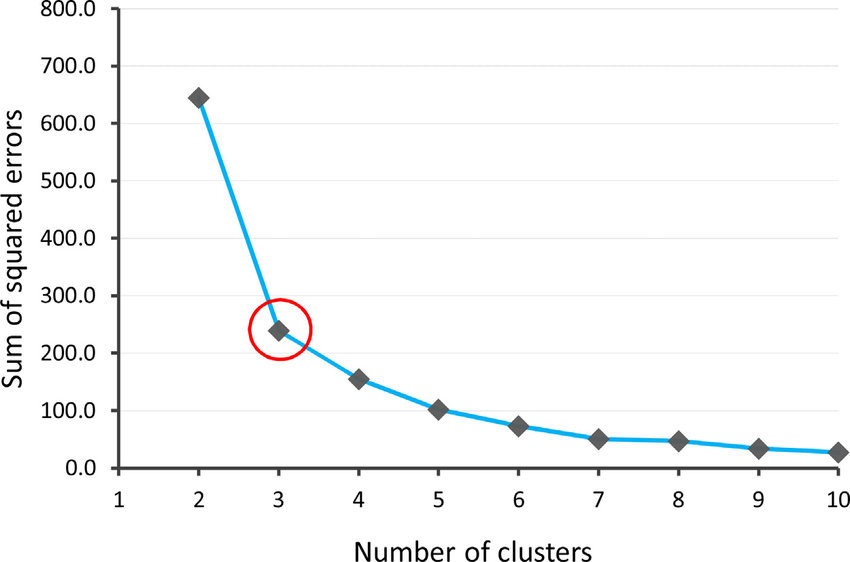
\includegraphics[width=0.7\textwidth]{Figures/elbow.png}
    \caption{Elbow method for k-means clustering}
    \label{fig:elbow}
\end{figure}
However, the limitation of this method is that the elbow point cannot always be unambiguously identified - sometimes there is no elbow, or sometimes there are several elbows.

\subsubsection{Misclassification Error (ME) Distance}\label{condundrum2}

ME distance is used to calculate the similarity between two different clusterings of the same data. Given the "ground truth" (i.e. true classes of each point), we can compare the clustering obtained by our technique with the ground truth to see how our model compares. ME distance thus represents the well known cost of classification, minimized over all permutations of the labels \cite{meila2005comparing}. 

It is calculated as follows :-

Consider two clusterings $\mathbb{C} =\{C_1,C_2,...,C_K\}$ and $\mathbb{C'} =\{C'_1,C'_2^,...,C'_{K'}\}$. 
We define the confusion matrix of $\mathbb{C}$ and $\mathbb{C'}$ as a $K x K'$ matrix $M=[m_{kk'}]$, with $m_{kk'} = |\mathbb{C_k} \cap \mathbb{C'_{K'}}|$. We consider the case where both models cluster $N$ points, and $K=K'$. 

Then the ME distance is defined as
\begin{equation*}
    d(C,C') = 1 - \frac{1}{N} \max_{\pi \in \Pi_k} \sum_{k=1}^{K} {m_{k,\pi(k)}}
\end{equation*}
where $\Pi_k$ contains all permutations of the label $K$.

We want the ME Distance to be close to 0 for "better" clusterings.
\subsubsection{Gene Ontology}
Gene Ontology, Hierarchical Clustering - dendogram